\chapter{Key Infrastructure}
This chapter will present the concept of \gls{PKI} and \gls{IBE}, as well as problems and possible solutions. 

\section{Public Key Infrastructure}

X.509 (i.e. \gls{PKI}). Issues: certificates --> distribution and revocation.

\section{Identity-Based Cryptography}\label{ibc}
\gls{IBE} was first proposed by Shamir~\cite{DBLP:conf/crypto/Shamir84} in 1984. 
The concept of \gls{IBE} builds upon every user having an \gls{ID} that is used as the public key. 
This \gls{ID} can be anything, i.e. email, phone number, \gls{SSN}, or a Name (~\autoref{name}).
This eliminates the need of certificates.
Shamir did propose a scheme for \gls{IBS}, but not a scheme for \gls{IBE}. 
The \gls{IBE} implementation remained unsolved until 2001, when Dan Boneh and Matthew K. Franklin proposed~\cite{DBLP:conf/crypto/BonehF01}.
However the scheme has only been shown to be secure with a random oracles model~\cite{DBLP:journals/iacr/Waters04}, hence less practical.


\gls{IBE} is based upon performing cryptography with a publicly know \gls{ID}.
Since the \gls{ID} can be practically anything it is highly applicable for \gls{NDN} where the \gls{ID} can be a Name (``/ndn/no/ntnu/haakon'').
Hence the Name becomes the public key. 

There is a \gls{TTP} in \gls{IBE} that is called \gls{PKG}.
The \gls{PKG}s task is to produce a private key that corresponds to a given ID and provide 

\begin{enumerate}
  \item Setup generates a key pair, \gls{MPK} and \gls{MSK}. These keys are used to extracting private keys, encryption and decryption.
  \item Extract generates a private key from a given ID. 
  \item Encrypt(\gls{MPK}, ID, message)
  \item Decrypt(\gls{MPK}, private key, cipher)
  \item Signing(\gls{MPK}, private key, message)
  \item Verify(\gls{MPK}, ID, message, signature)
\end{enumerate}

\todo{figure of PKG and nodes}

Thoroughness of the name allocation \gls{NRS} 
Identity-based cryptography~\cite{DBLP:conf/icnp/ZhangCXWSW11} in \gls{NDN}

Key Revocation in IBE ~\cite{DBLP:journals/iacr/BoldyrevaGK12} 

To encrypt a message with \gls{IBE}, the user encrypts a \gls{CEK} with the recipients \gls{IBE} public key.
Then the user encrypts the message with the \gls{CEK}~\cite[section 2.2.2]{rfc5408}

Some drawbacks related to \gls{IBE} are listed below:
\begin{enumerate}
	\item If \gls{PKG} is compromised. Adversary has private key to all nodes that used the compromised \gls{PKG}
	\item \gls{PKG} can read and write messages related to the node, because it has all private keys, i.e. \gls{MITM}.
	\item \gls{PKG} and the requesting node has to establish a secure channel. 
\end{enumerate}

\section{Key Distribution}
Instead of in \gls{PKI} where each public key is signed by a certificate authority and the generated certificate is sent as a response in \gls{HTTPS} then validated by the the client, we want to make the certificate authority obsolete by distributing every \gls{ID} (public key) issued by the \gls{PKG}.
This can be done through an IDSync application built upon the application presented in~\autoref{file-sync}.
In~\autoref{fig:pkg_sync} we see that the \gls{PKG} multicasts the \gls{ID} list to all devices that have joined the domain.
Each device can verify the integrity and authenticity of the sync state Data and be sure that the \gls{ID} list surely originates from its own \gls{PKG}.
\begin{figure}[H]
  \centering
  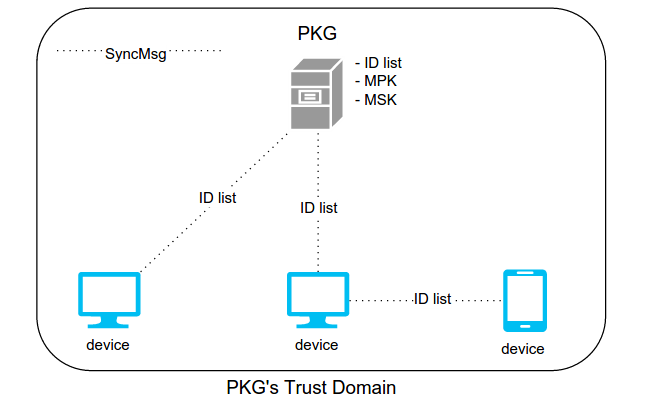
\includegraphics[width=1\textwidth]{pkg_sync.png}
  \caption{IDSync with tree devices and a \gls{PKG}.}
  \label{fig:pkg_sync}
\end{figure}

\section{Key Revocation}
Few alternatives to revocation scheme in \gls{IBE}.
One suggestion is to allocate private keys with the public key combined with some sort of date, e.g. month-year or just year. 
In this alternative a user has to renew its private key each time the date changes, i.e. either the month or the year depending on the date format.
The problem with the revocation solution is that it is cumbersome for the \gls{PKG}.


Key revocation becomes obsolete with the IDSync distribution solution. 
